To tend to this challenge, the team has decided to work with the
Kanban method, Kanban is a workflow management method that helps organization
manage and improve work systems, it originated in Japan. Firstly used by Toyota
as a scheduling system for just-in-time manufacturing, it was later adopted by
many other organizations to take toll on software industry in the 21st century, 
it's a flexible and agile method that can be used in many different situations,
for more information \cite{kanban_def}.


The tasks were divided into the following categories:
\begin{itemize}
    \item Stand-By: For non-urgent tasks, or that are not ready to be worked on.
    \item Requested: For tasks that are ready to be handled.
    \item In Progress: For tasks that are being worked on.
    \item To Review: For features or tasks that were done,
        and should be either reviewed or tested.
    \item Done: For tasks that have been completed.
\end{itemize}

\begin{figure}[!htpb]
    \centering
    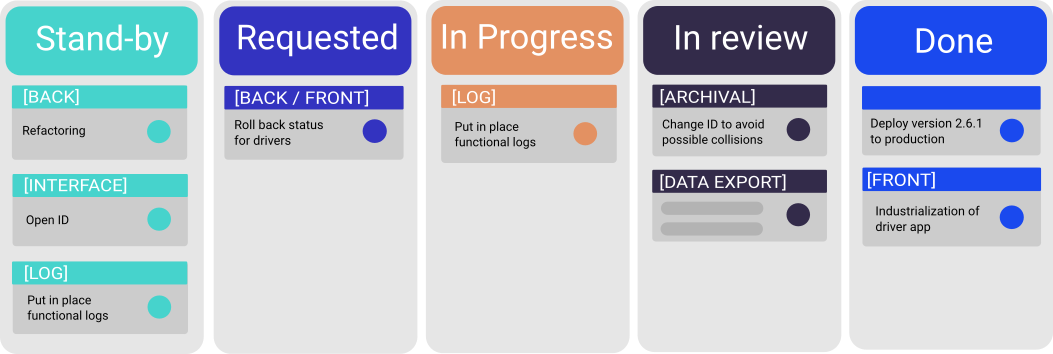
\includegraphics[width=\textwidth]{images/kanban_mod.png}
    \caption{\footnotesize{Kanban board elements}}
    \label{fig:kanban-board-elements}
\end{figure}

The board was handled using Jira, which is a web-based project management tool developed
by Atlassian that is used to track and manage the development of software projects,
allowing for a wide range of flexibility within the application.

Choosing the features to be implemented in the system was a challenge,
as there were specifications to be followed, and the requirements were
kind of wild and not realistic for the given time frame.

So prior to beginning on the kanban board, there were a few meetings 
mainly to discuss features within the specifications which were to be implemented 
in the system and which were to be kept on hold.

The creation of the tasks then was handled either by the product owner or the project
manager, and giving each one a priority, and a due date was assigned once the task was
picked up and studied for the implementation to assess the proper manner to handle it.

For the reviewing of the tasks, it was decided to be moved to done once the task was
tested thoroughly by the product owner trying to find any issues that may have
passed through the testing done by the developers.

\begin{figure}[!ht]
    \centering
    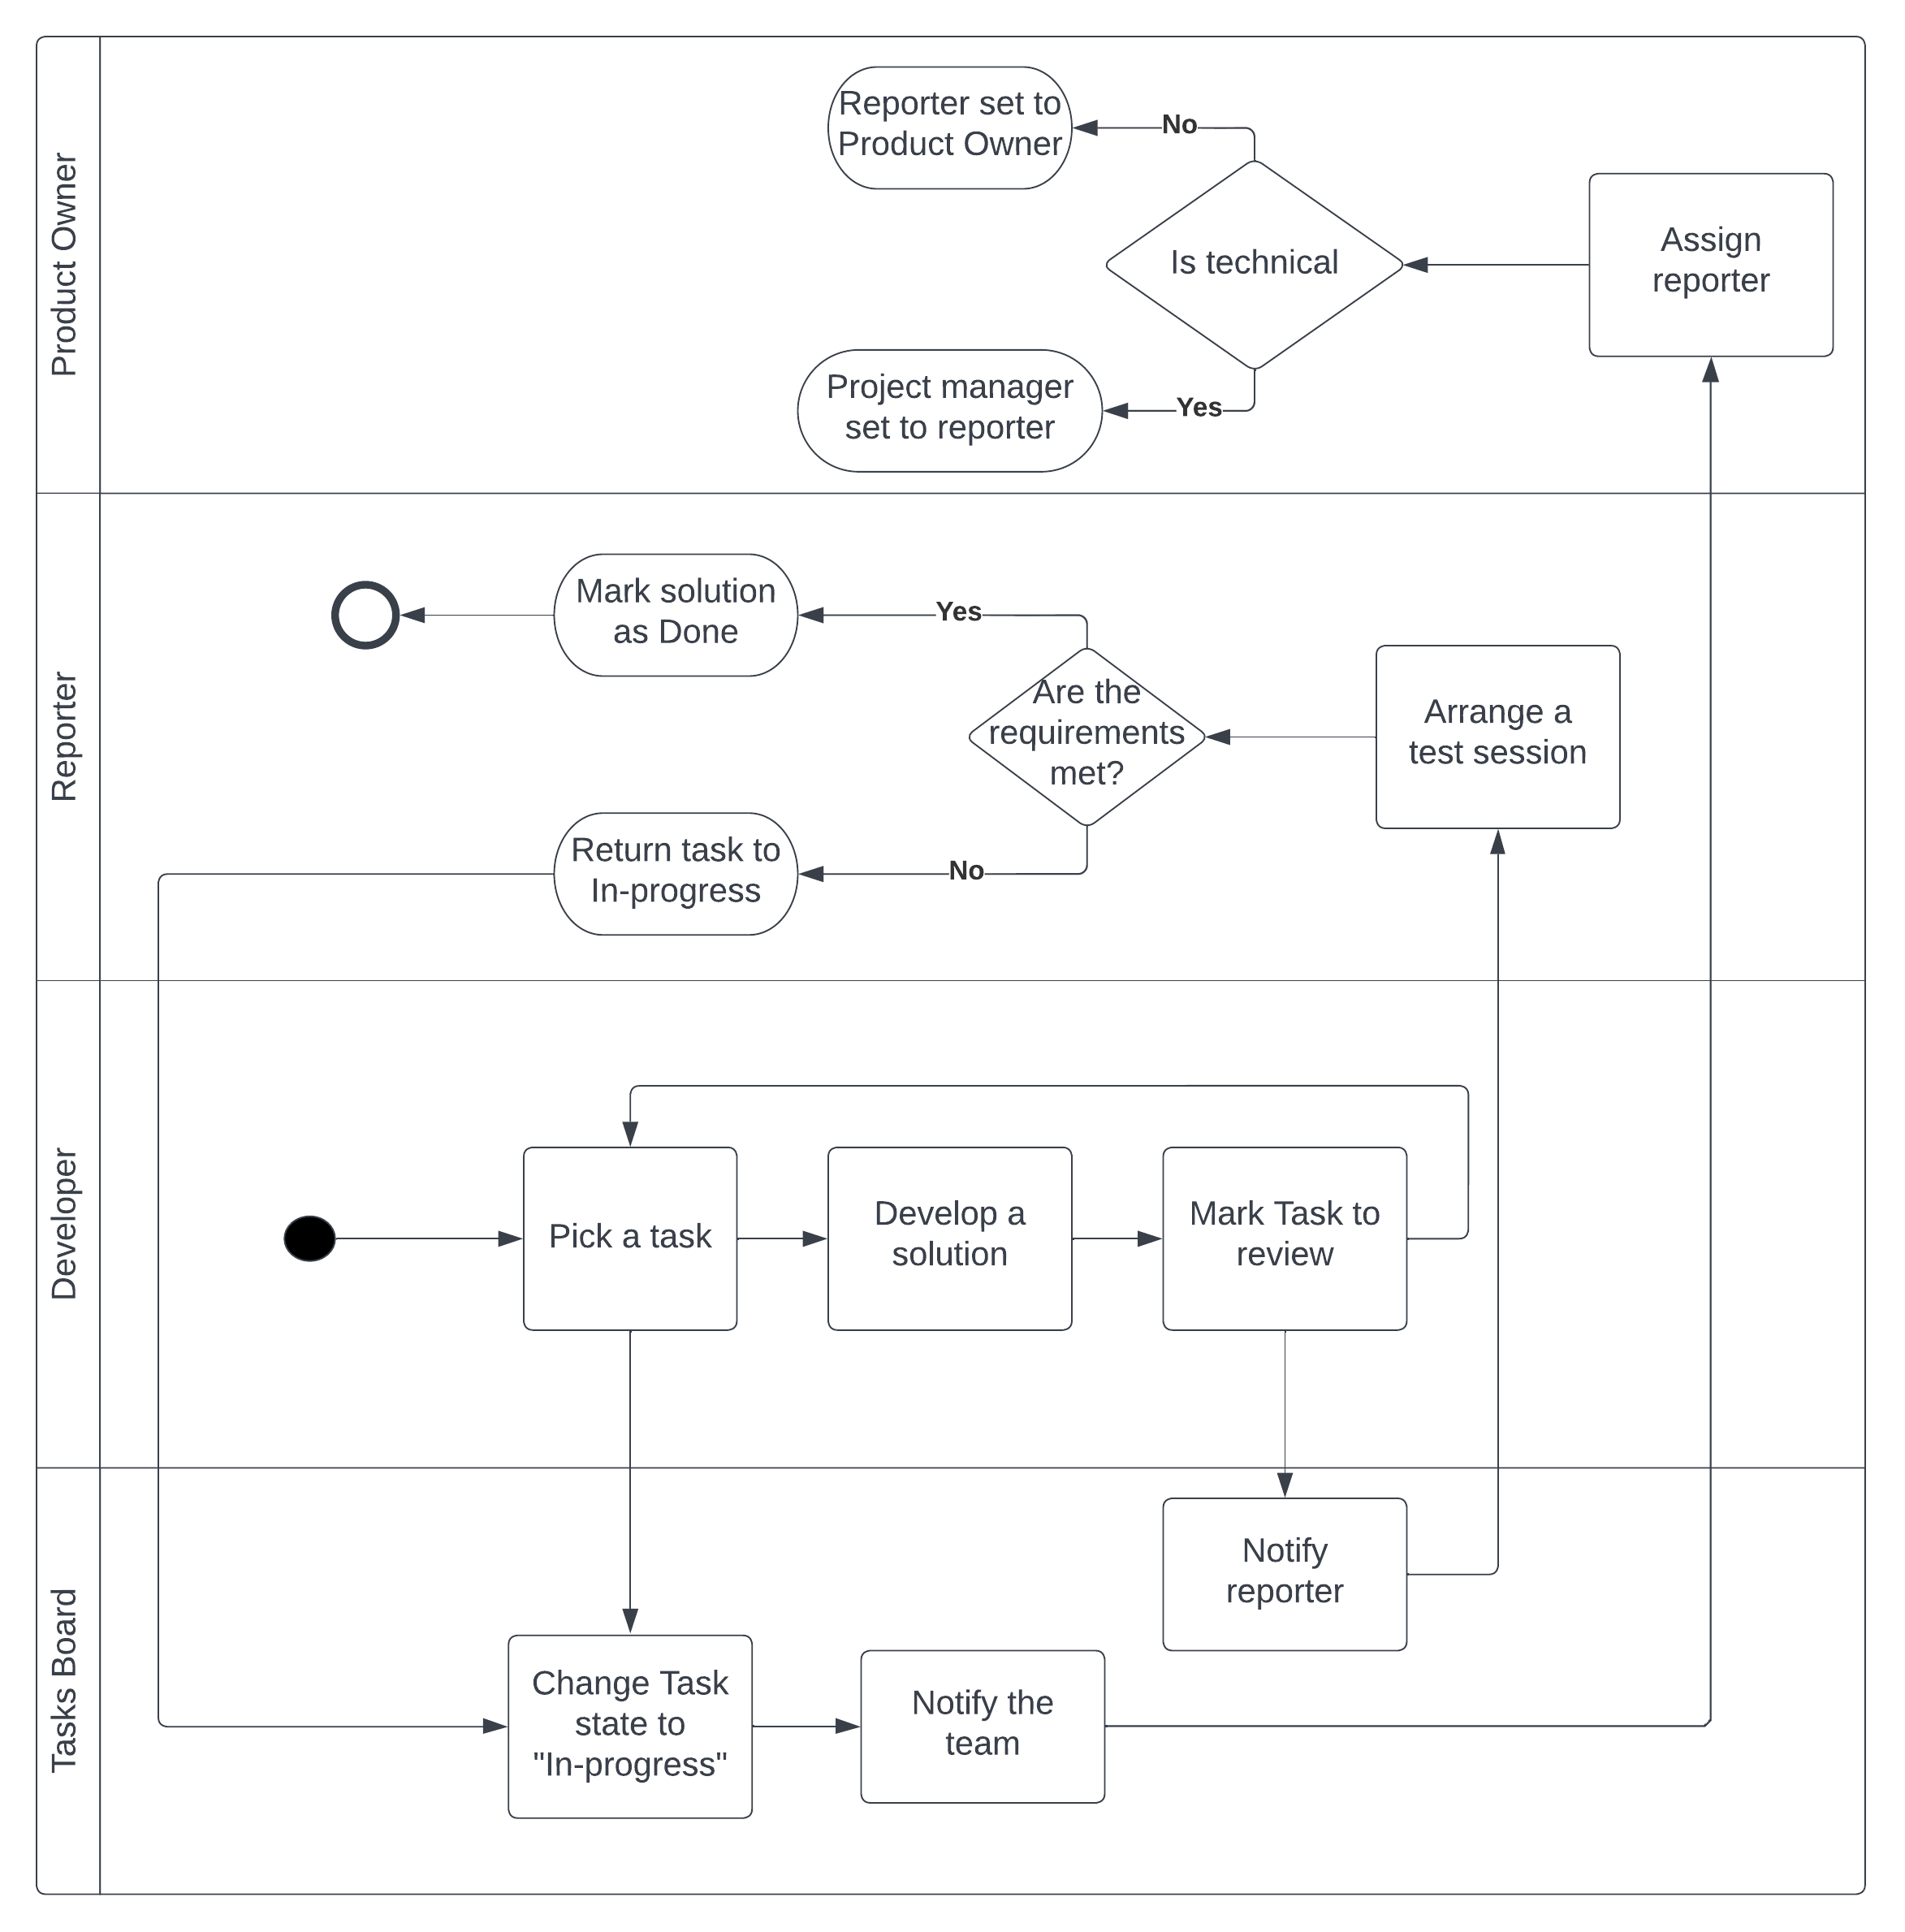
\includegraphics[width=\textwidth]{images/task handling flow.png}
    \caption{\footnotesize{Task handling - flow chart}}
    \label{fig:task_handling}
\end{figure}

During the development the tasks handling went as showing in figure \ref{fig:task_handling}
and the order was as follows:
    \begin{itemize}
        \item Pick up the task from the requested list.
        \item Task get assigned to the developer who picked it.
        \item Task is moved to the in progress list.
        \item Once done the task is moved to the to review list.
        \item Once reviewed the task is moved to the done list.
    \end{itemize}

For the reviewing of the tasks, it went in two ways, one for the product owner to
review the task when it's related to some business logic or frontend interactive task
and the other for the CTO to review the ones relating to the backend logic and purely,
technical tasks.

\begin{sidewaysfigure}
    \centering
    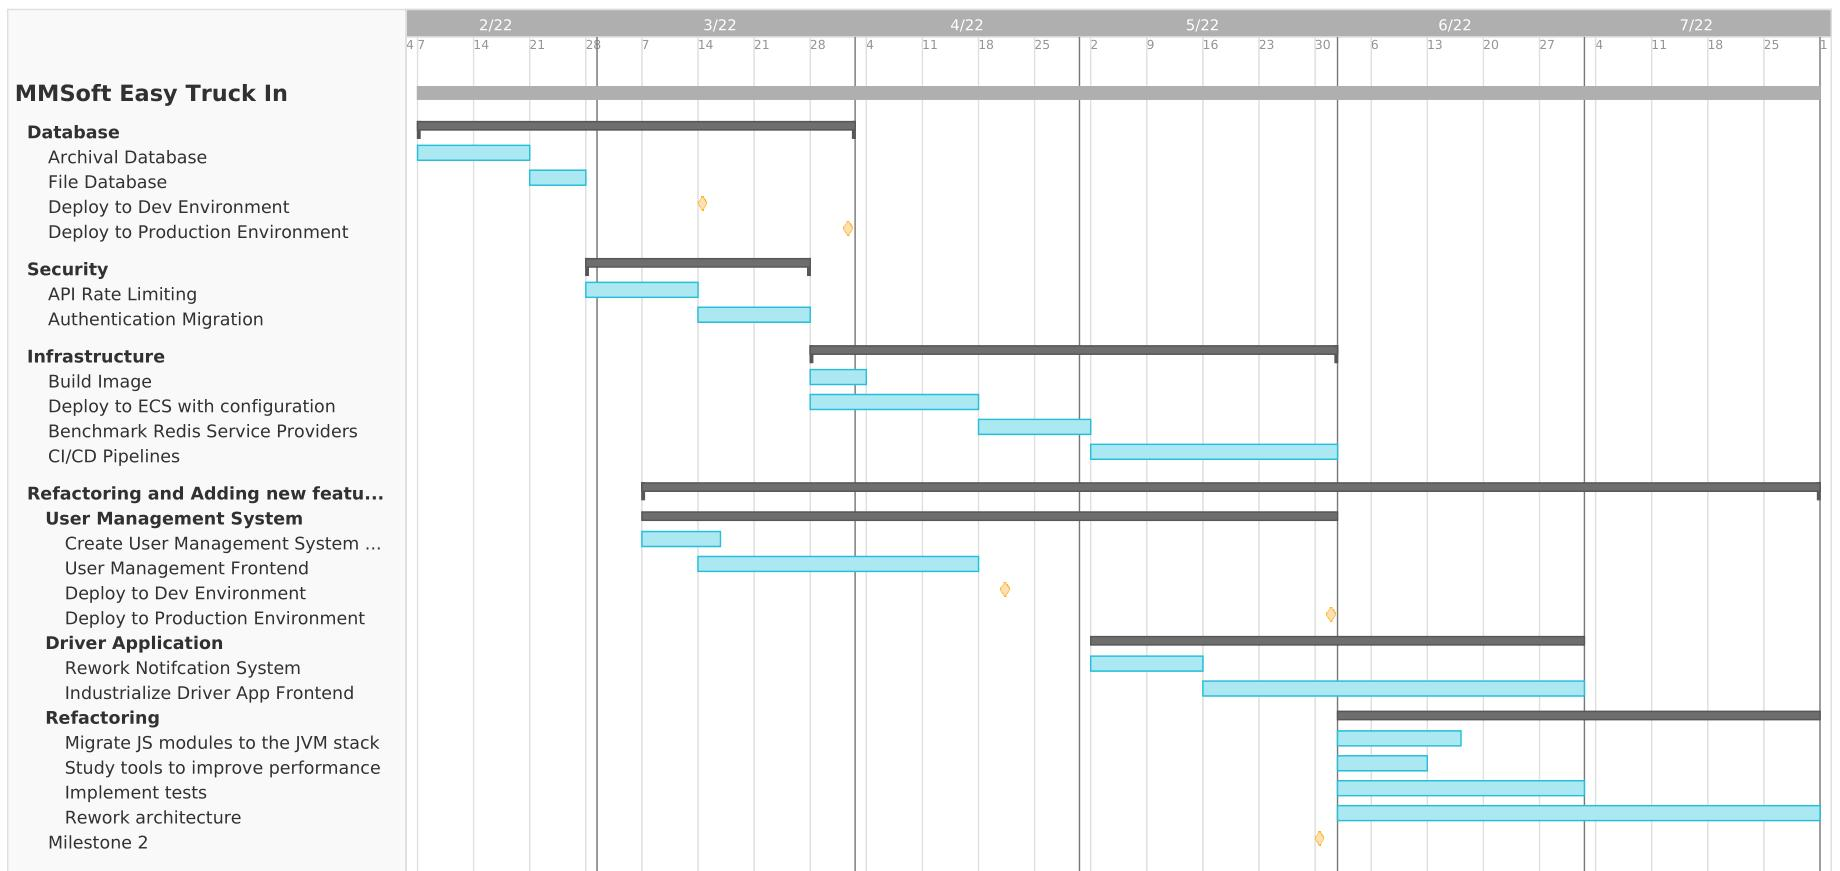
\includegraphics[width=\textwidth]{images/Plan.jpeg}
    \caption{\footnotesize{Gantt chart of the project}}
    \label{fig:gantt_chart}
\end{sidewaysfigure}

For the forecast plan, it had multiple tasks and milestones planned out as shown in the
\newline figure \ref{fig:gantt_chart} there is the following:

\begin{itemize}
    \item Databases: The solution required specific new features related to data
        to implement. The first one being archival of clients data,
        and the second is the ability to store files and both these
        came with a cost for storage in mind.
    \item Security: Which had multiple layers of security to be handled,
        one of them was handling the authentication of the users to make it
        less exploitable, the other managing the access to the system and
        last rate limiting the api gateway.
    \item Infrastructure: The solution required a new infrastructure, specifically
        one that would allow for the deployment of the system in streamlined
        manor, and also the ability to scale the system through peak times.
    \item New Features: The solution required new features to be implemented,
        which were not a nice to have but rather a necessity, and these were
        addition of a User management system and notification system.
    \item Refactoring and testing: as discussed before the solution came as an
        MVP which required refactoring and testing to be done.
        This part came with a lot of work in mind, firstly a studying of the
        existing tools and libraries to be used, and compare them to the already
        used ones, also the code base was missing a lot of tests for the exisitng
        features so it needed a to have every part of the code have it's own
        tests implemented to ensure the consistency of the behaviour.
        And finally, a rethought architecture of the code base to make it 
        more future-proof and maintainable.
\end{itemize}

\section{Conclusion}

To sum up we've discussed so far the scope of the project, which is taking place
within the "ONAR MMSoft" company, specifically within their product Easy Truck In (ETI)
which is a software application that is used to manage the trucks in warehouses.
The problem with this product is that it's still just a PoC at the moment and they 
are planning to expand their product to a wider audience, which would necessitate 
making it more robust and scalable product, specifically one that would be following
industrial SaaS standards and standards for the software industry.
